\documentclass[12pt]{beamer}
\usepackage{mathtools}
\usepackage{makecell}
\useoutertheme{infolines}
\usetheme{default}
\usefonttheme{serif}
%\usefonttheme{structuresmallcapsserif}
\hypersetup{colorlinks=true,linkcolor=blue}
\setbeamertemplate{navigation symbols}{}
\author{Mittereder, \textit{et. al.}}
\definecolor{darkgreen}{rgb}{0,.5,0}
\setlength{\parskip}{.1in}

\begin{document}

\begin{frame}[c]{} % Justin

\begin{center}
\Large
Exploring the Impact of Social Network Density\\and Agent Openness on Societal Polarization

\footnotesize
\vspace{.3in}
CSS 2021 --- Santa Fe, New Mexico (sorta)\\
\vspace{.1in}
Justin Mittereder, Robert S.~W.~Carroll, Brandon Frulla, Stephen Davies\\
\scriptsize
\smallskip
Dept of Computer Science\\
University of Mary Washington\\
Fredericksburg, Virginia, USA\\
\end{center}

\end{frame}

\begin{frame}[c]{Defining polarization} % Stephen

\large

\centering
``America is becoming increasingly polarized..."

\vspace{-.2in}
\begin{figure}
\includegraphics[width=0.50\textwidth]{images/capitol.png}
\end{figure}
\pause
\vspace{-.2in}
What does this actually mean?
\vspace{-.15in}
\pause

\small
\begin{itemize}
\itemsep.1em
\item People's views becoming more \textit{extreme}?
\pause
\item People becoming more \textit{stubborn}? (less willing to reconsider views)
\pause
\item People only associating with like-minded others?
\end{itemize}

\end{frame}

\begin{frame}[c]{Polarization Proxy \#1: Assortativity coefficient} % Justin

% TODO: add slides from extravaganza, and explain assortativity well

% explain why we think this is a measure of polarization

% "echo chambers"


\begin{figure}
	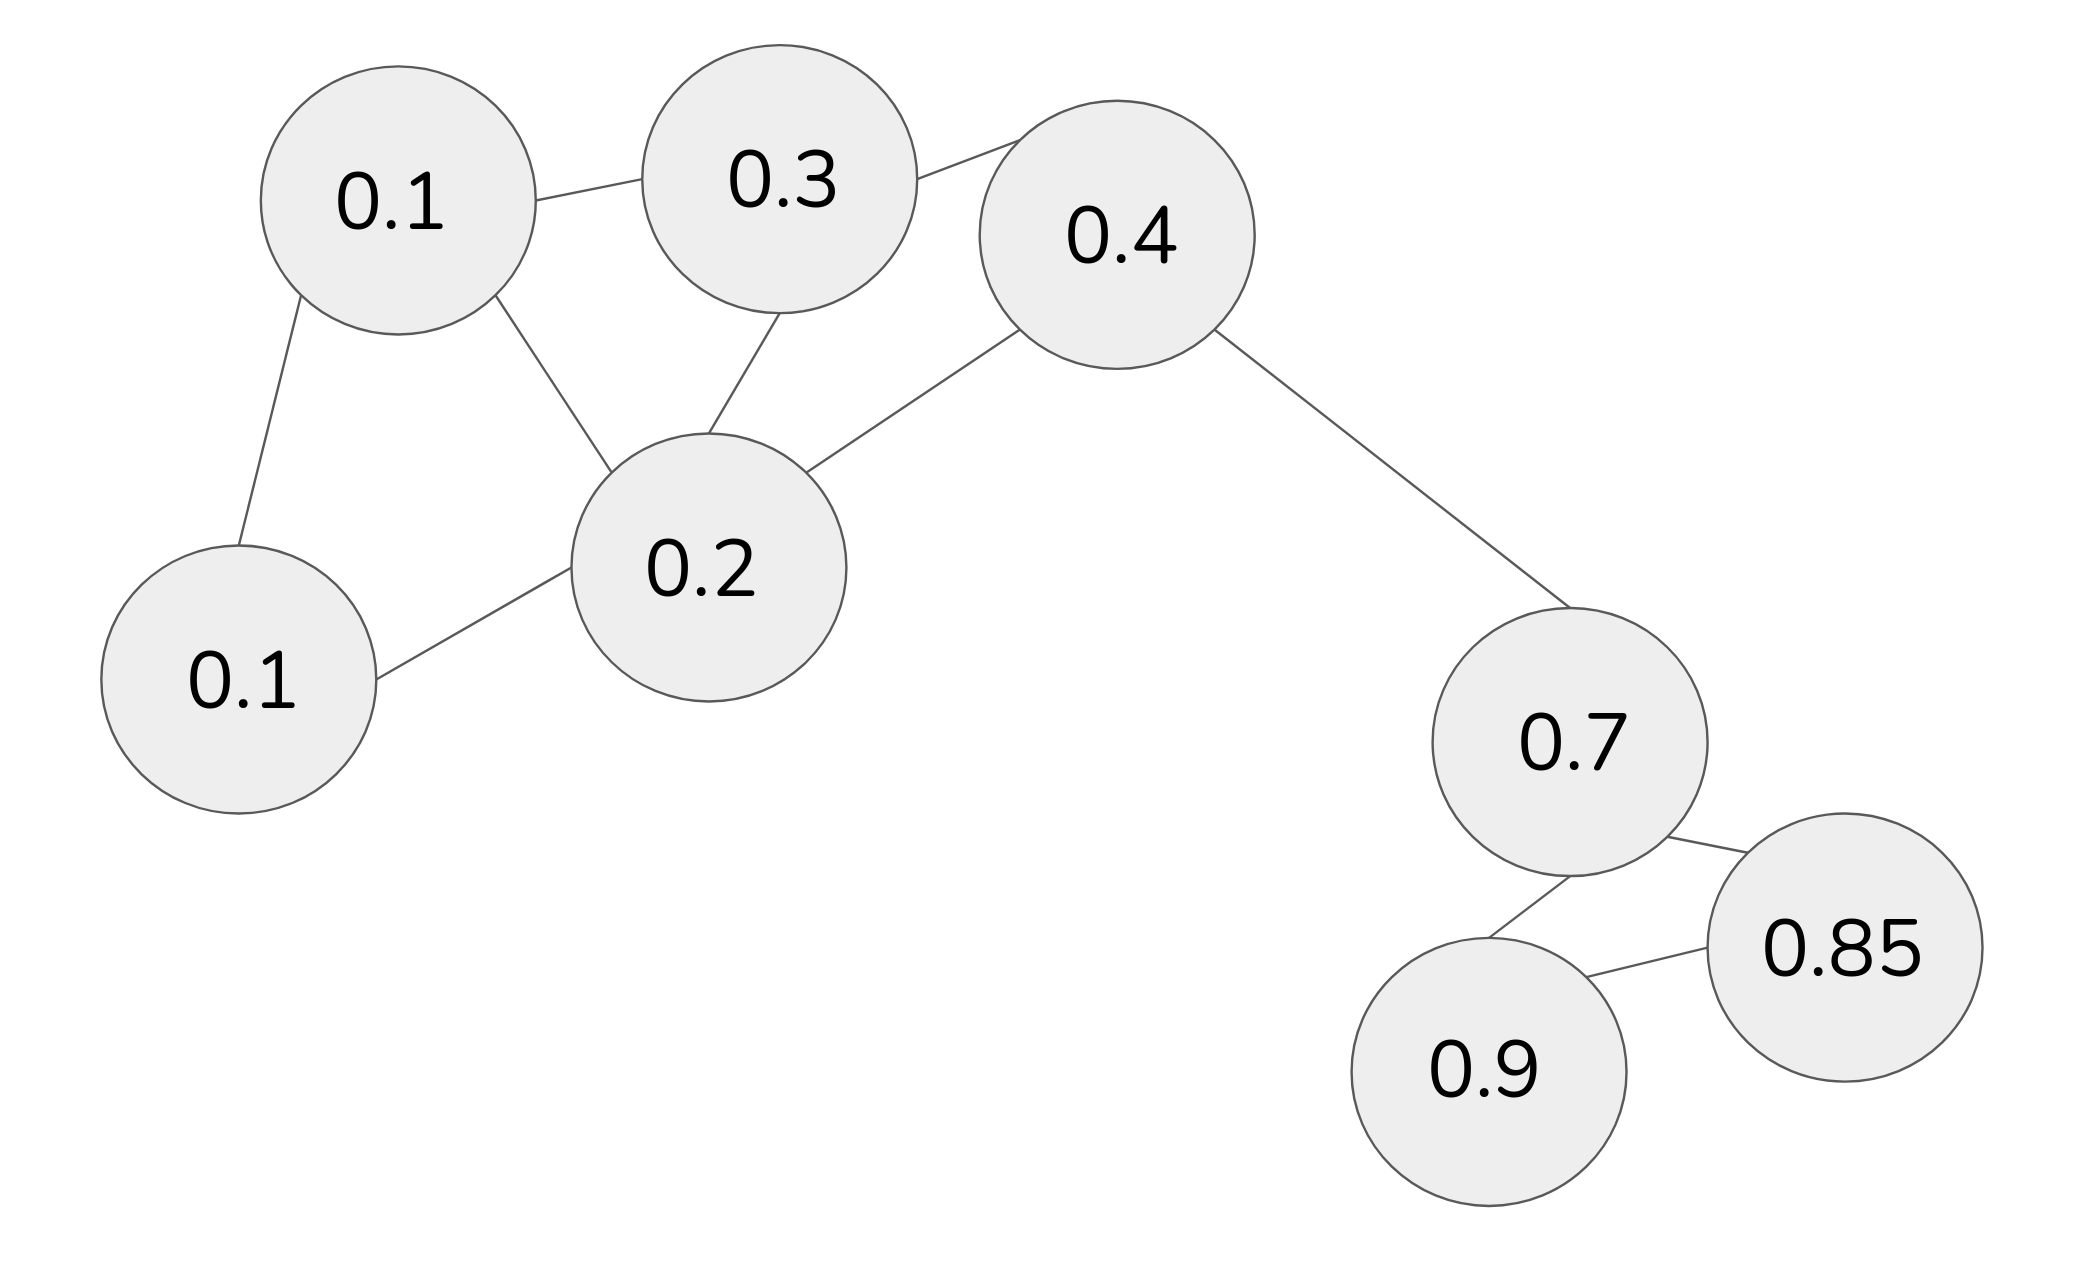
\includegraphics[width=0.40\textwidth]{images/HighAssortDiagram.png}
	\hfill
	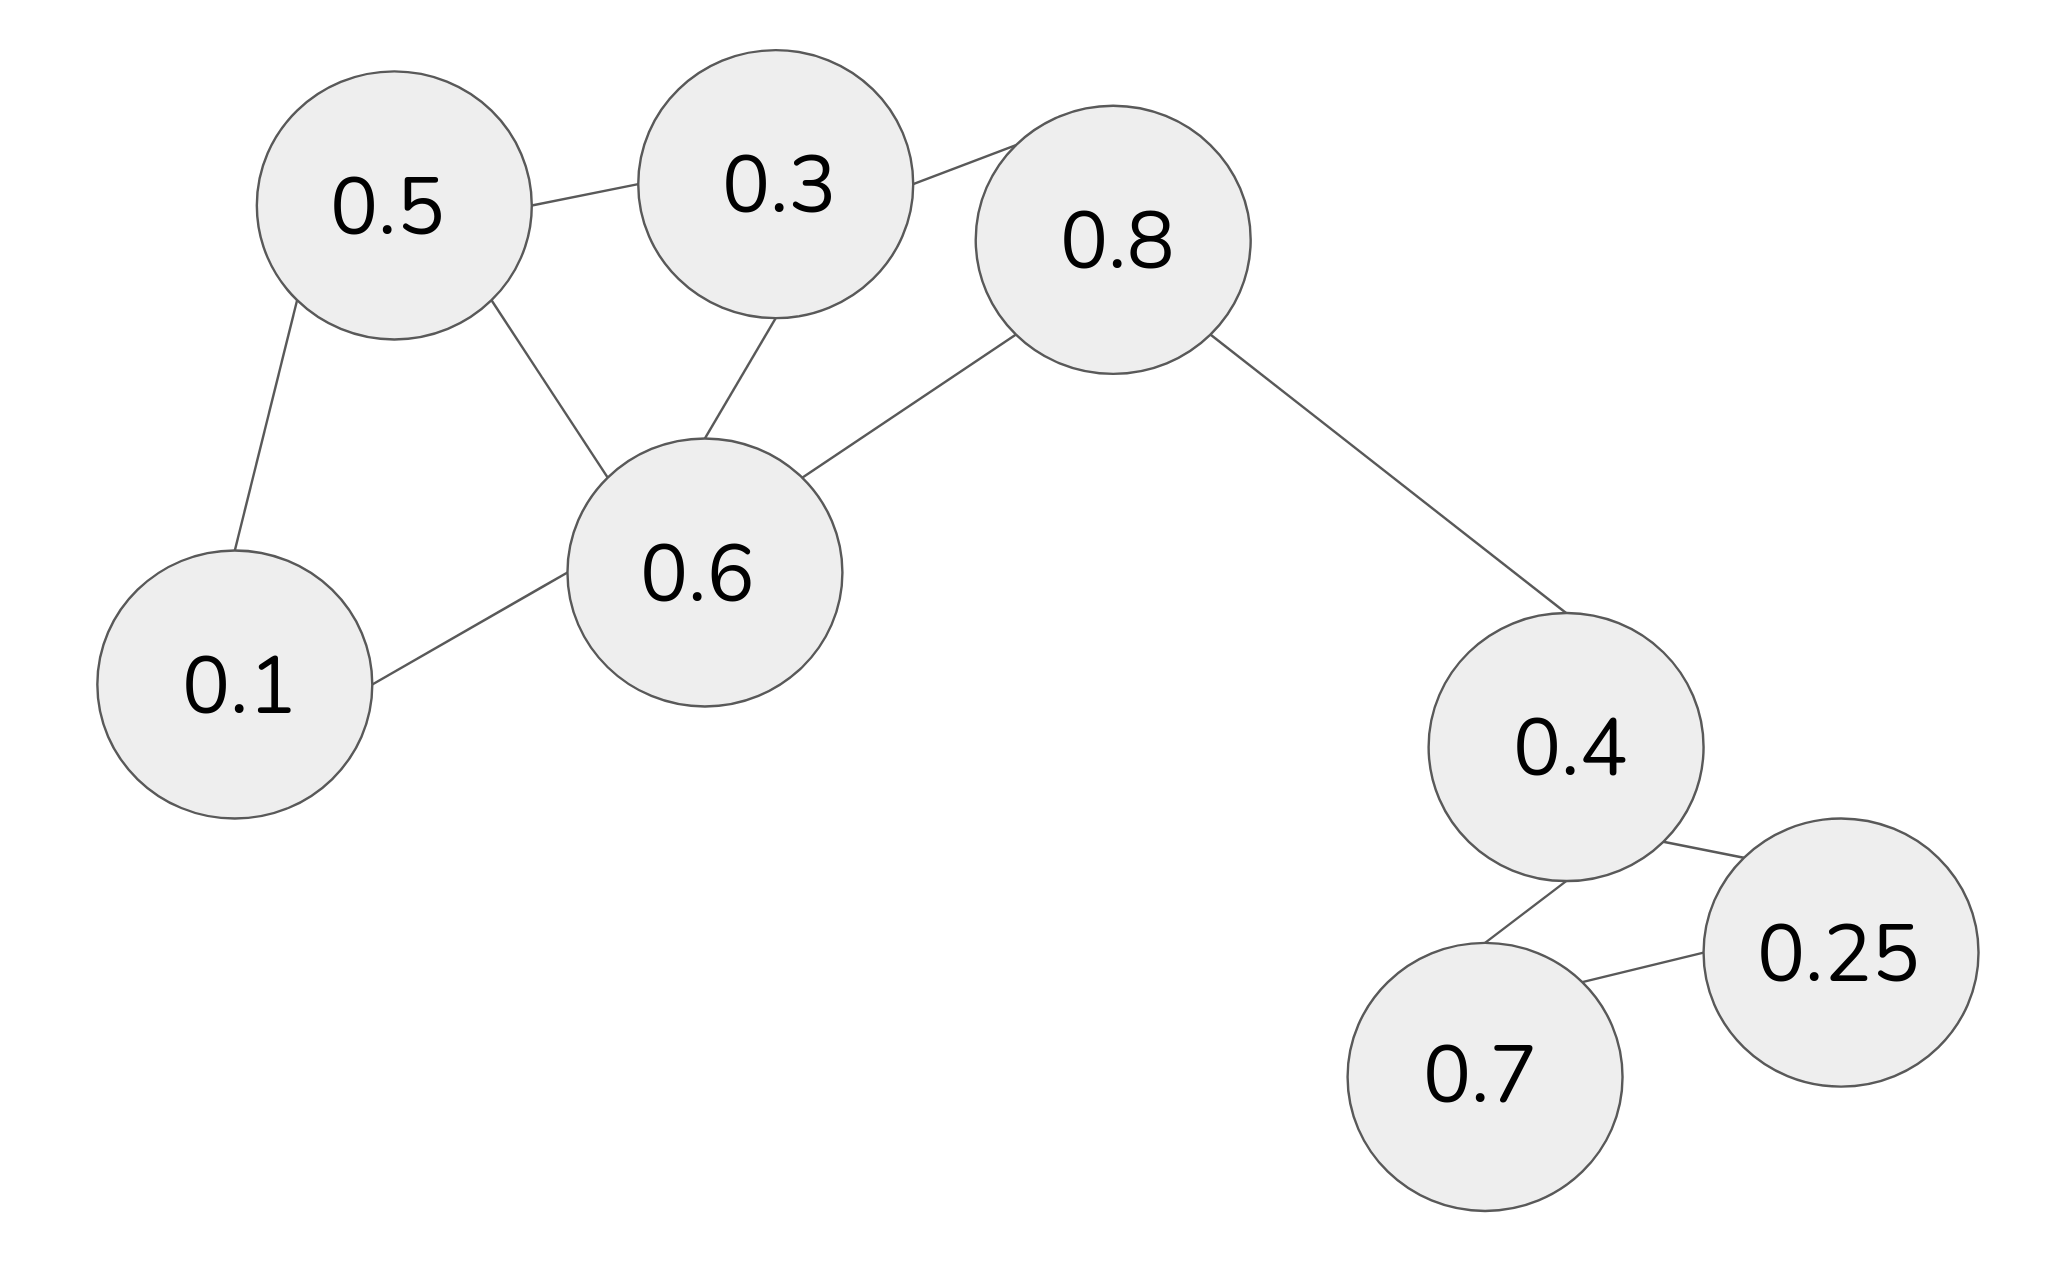
\includegraphics[width=0.40\textwidth]{images/LowAssortDiagram.png}
	%TODO: add captions for high and low assort
\end{figure}

\end{frame}


\begin{frame}[c]{Polarization Proxy \#2: Issue Alignment} % Stephen

We define \textbf{Issue Alignment} (IA) as the tendency for people who agree on
one issue to also agree on other (unrelated) issues.

\begin{center}
\begin{tabular}{c|c}
\pause
raise the minimum wage & lower the minimum wage \\
\pause
pro-choice & pro-life \\
\pause
higher taxes \& services & lower taxes \& services \\
\pause
anti-guns & pro-guns \\
\pause
pro-immigration & anti-immigration \\
\pause
pro-vaccine-mandate & anti-vaccine-mandate \\
\pause
pro-renewable-energy & pro-fossil-fuels \\
\pause
... & ... \\
\end{tabular}
\end{center}

\pause
\footnotesize

If people generally adhere to an entire suite of opinions, we term that society
``Issue Aligned'' and claim this is an indication of polarization.

\end{frame}

\begin{frame}[c]{The model}  % Justin

% Describe in selected detail the model

% N heterogeneous agents who encounter each other on a social network.

% ER edge prob is a parameter

% Multiple continuous opinions 
\large

\centering
Opinion Dynamics ABM

\vspace{.05in}
Model Characteristics:
\vspace{-.15in}

\small
\begin{itemize}
\itemsep.1em
\item \textit{N} heterogenous agents who encounter each other on a social network.
\item \textit{Edge Probability} of a random Erd\"{o}s-R\'{e}nyi graph which controls network density
\item Agents have multiple opinions that exist on a continuum
\item \textit{Openness Threshold} and \textit{Disgust Threshold} that control the degree of agent opinion influence
\end{itemize}


\end{frame}


\begin{frame}[c]{Traditional BC with Positive Influence}  % Justin

% Here is traditional bounded confidence (BC) from Hegelsmen-Krause and
% Deffuant et al

% Show one number line and two peeps
\begin{figure}
	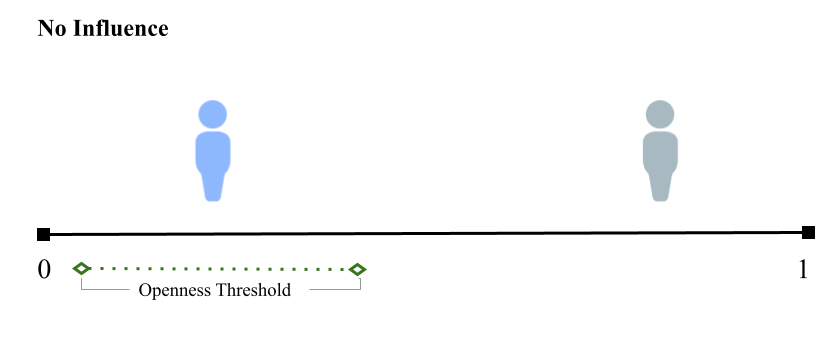
\includegraphics[width=0.65\textwidth]{images/BCNoInfluence.png}
	\hfill
	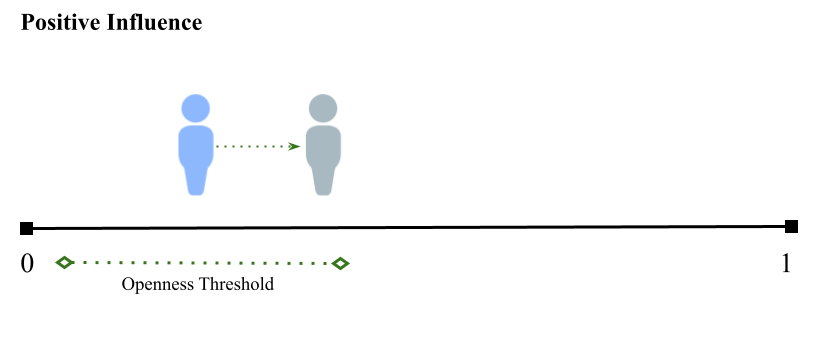
\includegraphics[width=0.65\textwidth]{images/BCPositiveInfluence.png}
	%TODO: add captions
\end{figure}


\end{frame}

\begin{frame}[c]{Traditional BC with Negative Influence}  % Justin

% Here is traditional bounded confidence (BC) from Hegelsmen-Krause/Deffuant with repulsion

\begin{figure}
	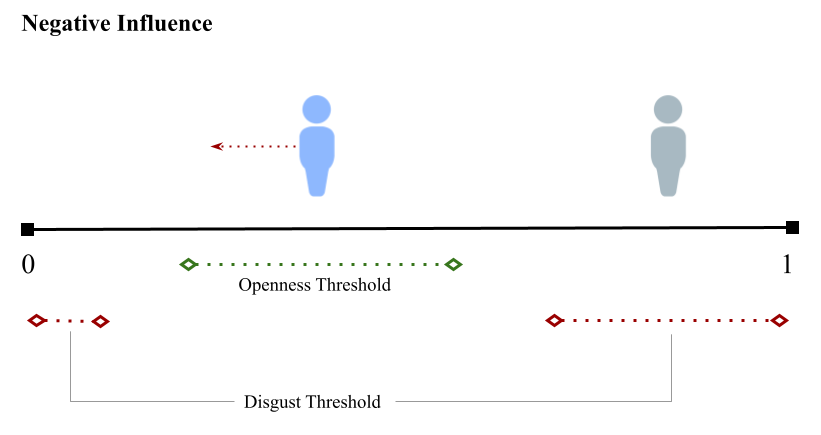
\includegraphics[width=0.65\textwidth]{images/BCNegativeInfluence.png}
	%TODO: add captions
\end{figure}


\end{frame}

\begin{frame}[c]{Cross-Issue Influence (Positive only)}  % Justin

% Show two number line and two peeps, with an attraction due to openness
We define \textbf{Cross-Issue Influence} (CI2) as the effect that a person's
social contact can have on one of their opinions based on their agreement (or
disagreement) on a different issue.

\begin{figure}
	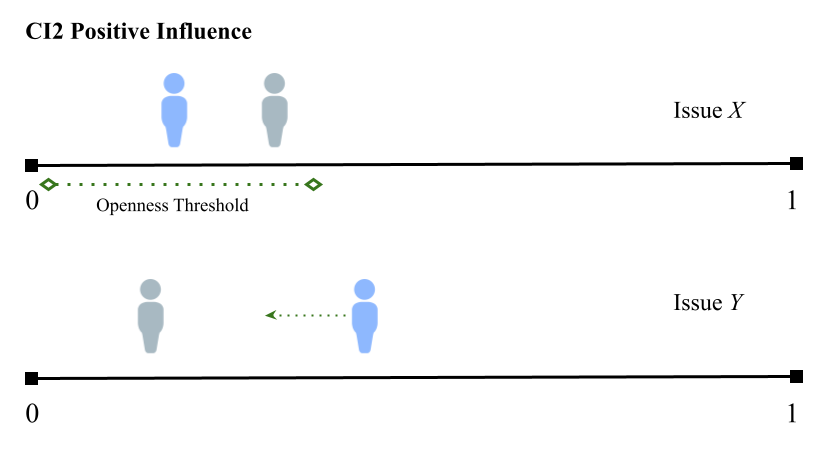
\includegraphics[width=0.75\textwidth]{images/CI2Attraction.png}
	%TODO: add captions
\end{figure}

\end{frame}


\begin{frame}[c]{Cross-Issue Influence (adding Negative)}  % Justin

% Show two number line and two peeps, with a repulsion due to disgust

% Also show the Justin threshold diagram with red & green regions

% And cite Griffin, Em (2011). A First Look at Communication Theory. New York,
% New York: McGraw Hill. pp. 194–204.
\begin{figure}
	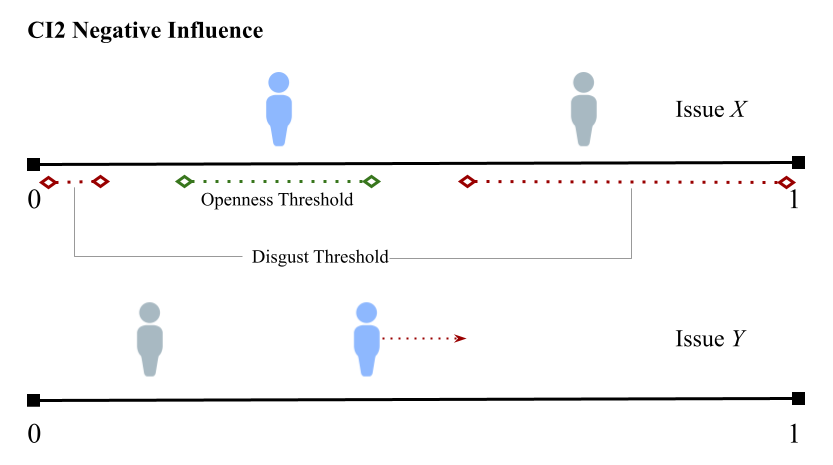
\includegraphics[width=0.75\textwidth]{images/CI2Repulsion.png}
	%TODO: add captions
\end{figure}

\end{frame}

\begin{frame}[c]{Fig 1 explained}  % Justin

Fewer (meaningful) social connections = higher polarization BUT only at the low
end.

\end{frame}

\begin{frame}[c]{Fig 2 explained}  % Justin

%TODO: Justin verify
%(Just for completeness, rerun paper graph Figure 2 with a much lower value of
%edge prob (how about .05 instead of .5, for instance.) Then we’ll verify the
%null hypothesis that “openness does not impact assortativity.”)

openness threshold surprisingly does not seem to impact assortativity.

\end{frame}

\begin{frame}[c]{Issue Alignment (IA)} % Stephen

%\textbf{Issue Alignment} (IA): the tendency for people who agree on one issue
%to also agree on other (unrelated) issues.

\textit{Why} does IA occur?

Possible explanation \#1: perhaps there is some deep underlying
principle to people's ideologies that connects seemingly unconnected issues.
\pause

\begin{center}
\begin{tabular}{clp{1cm}rc}
\makecell{
\\

\includegraphics[width=0.15\textwidth]{thinker1.jpg}
} &
\makecell{
Ideology 1 $\Rightarrow$ \\
Opinion A \\
Opinion B \\
Opinion C \\} & &
\makecell{
Ideology 2 $\Rightarrow$ \\
Opinion D \\
Opinion E \\
Opinion F \\} &
\makecell{
\\

\includegraphics[width=0.1\textwidth]{thinker2.jpg}
}
\end{tabular}
\end{center}

\end{frame}

\begin{frame}[c]{Issue Alignment (IA)} % Stephen

\textit{Why} does IA occur?

Possible explanation \#2: perhaps a small number of popular media
outlets each articulates a set of opinions on various issues. 

\pause
\begin{center}
\begin{tabular}{clp{1cm}rc}
\makecell{
\\

\includegraphics[width=0.15\textwidth]{listener1.jpg}
} &
\makecell{
News source 1:  \\
``Opinion A!'' \\
``Opinion B!'' \\
``Opinion C!'' \\} & &
\makecell{
News source 2:  \\
``Opinion D!'' \\
``Opinion E!'' \\
``Opinion F!'' \\} & 
\makecell{
\\

\includegraphics[width=0.15\textwidth]{listener2.jpg}
}
\end{tabular}
\end{center}

%The people who
%listen to them are naturally influenced to each of these different opinion
%values, and thus become ``issue aligned."

\end{frame}

\begin{frame}[c]{A third possible explanation for IA} % Stephen

CI2!

{\tiny \color{red} 
Stephen TODO:

We wish there was more justification in the social psych lit for this, but we
have to fall back on (1) homophily and (2) common sense.
}

{\small \color{red} 
Big idea: even without any underlying ideological connection between issues,
and even without media influence, IA will naturally develop solely due to CI2.
In other words, CI2 is sufficient for IA. (Wide reaching implications on how we
interpret the causes of the polarization phenomenon, and what societal changes
might be necessary to reduce it.)
}

\end{frame}

\begin{frame}[c]{IA example} % Stephen

\end{frame}


\begin{frame}[c]{Define "buckets"} % Stephen

\end{frame}


\begin{frame}[c]{Define "clone pair" / anti-clone pair} % Stephen

\end{frame}



\begin{frame}[c]{Census plot w/o CI2} % Stephen

\end{frame}

\begin{frame}[c]{Census plot w/ CI2} % Stephen

\end{frame}

\begin{frame}[c]{Heat maps: showing interplay of openness and disgust threshold
with and without CI2} % Stephen

\end{frame}


% Tuck-away slide
%\begin{frame}[c]{Diametricity}
%
%One other way to define polarization is extremity of views.
%
%Fact: if CI2 is employed, the model always (?) produces exactly two buckets,
%and all the opinions in those buckets are at the poles.
%
%Fact: if only I2 is employed, there will normally be many buckets (often one
%for each combination of fully-polarized opinions; i.e., a (0,0,0) bucket, a
%(0,0,1), (0,0,2), (0,1,0), ...)
%
%\end{frame}

\begin{frame}[c]{Discussion and takeaways}  % Stephen & Justin

\end{frame}

\begin{frame}[c]{}

\begin{center}
\Large
Exploring the Impact of Social Network Density\\and Agent Openness on Societal Polarization

\footnotesize
\vspace{.3in}
CSS 2021 --- Santa Fe, New Mexico (sorta)\\
\vspace{.1in}
Justin Mittereder, Robert S.~W.~Carroll, Brandon Frulla, Stephen Davies\\
\smallskip
\scriptsize
Dept of Computer Science\\
University of Mary Washington\\
Fredericksburg, Virginia, USA\\
\end{center}

\end{frame}
\end{document}
